\chapter{BDS and Final-Focus system as background sources}
\section{Background from a Beam Halo Collimator in Final-Focus system}
\subsection{Beam Halo Collimator}
Picture: Collimator drawing\\
Picture: Pictures of installed collimator
\subsection{ATF2}
Picture: ATF2 schematic
\subsection{BDSIM}
%---------------------------------------------------
\subsection{Background studies}
\subsubsection{RHUL Cherenkov detector}
Pictures: setup\\
\begin{figure}
\centering
\includegraphics[width=\textwidth]{AverageNoise_perVoltage.pdf}
\caption[RHUL Cherenkov detector noise]{Average noise signal as a function of the voltage applied to the detector PMT. The noise was measured when the ATF beam was turned off. For each voltage, 500 or 1000 ADC pulses of noise were recorded, and the noise averaged over the number of pulses. The error bars to the mean values are the standard deviation of the mean.}
\label{fig:AverageNoise}
\end{figure}
Figure ~\ref{fig:AverageNoise} shows the mean values of the noise measurements for different PMT voltages. For every point either 500 or 1000 ADC pulses were recorded and averaged. The error bars represent the standard deviation on the mean value calculated by $SD=\frac{\sigma}{\sqrt{N}}$, where $\sigma$ is the RMS of the noise distribution at each point and N the number of pulses.\\
At around \SI{800}{\volt} the effect of dark current in the PMT starts getting prominent wherefore the noise rises exponentially. For the data shown in the following, the noise is already subtracted. As the data was taken only for these voltages, for which noise measurements were done, the mean value of noise is subtracted from every signal pulse appropriately. Therefore the rise in noise is automatically taken into account for higher voltages.

\subsubsection{Collimator apertures scan - for different intensities and vacuum pressures}
The two jaws of the vertical beam halo collimator can be moved individually. Scans of the background for different collimator apertures were done, first for symmetric positions of the lower and upper jaw around the centre, later for asymmetric positions. Additionally, a scan was done with one jaw fully extracted and the other one moving to certain positions. The last scan is referred to as the 'half aperture scan', whereas the first two scans are the 'symmetric' and the 'asymmetric' scans.\\
Figure ~\ref{fig:AverageSignal_Aperture_BeamIntensities} shows the plot of the average detector signals for the asymmetric scan of different collimator apertures. The scans were done for five different beam intensities. It is clear that the background level rises with increase in intensity. The characteristic shape of the scan is however conserved: the background level is constant while closing the collimator from a full aperture of \SI{24}{\milli\metre} to about \SI{12}{\milli\metre}. When closing to \SI{10}{\milli\metre} the background level drops, and rises again when closing the collimator completely, i.e. to \SI{6}{\milli\metre} full aperture. This characteristic drop and rise between 12 and \SI{6}{\milli\metre} is on the one hand proof of the proper functionality of moving the collimator jaws, on the other hand leaves some questions open: where are the background particles originating that are cut away by the collimator, and does the rise in background mean that the collimator is showering the beam halo particles? Which qualities do these produced background particles have?\\
These questions are addressed in Chapter ~\ref{sec:BDSIM_sim}, in which the effect of the collimator is simulated in a BDSIM simulation.
\begin{figure}
\centering
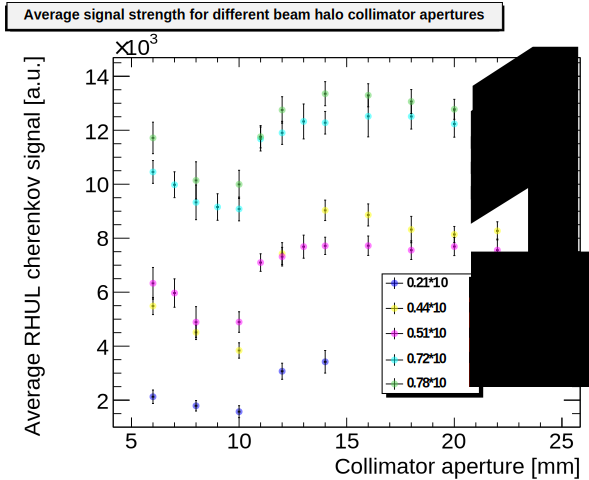
\includegraphics[width=\textwidth]{AverageSignal_perAperture.pdf}
\caption[RHUL Cherenkov detector signal vs. collimator aperture: different beam intensities]{Average signal as a function of the full aperture of the vertical beam halo collimator. The signal was measured for different beam intensities [\num{10e10}]: 0.21, 0.44, 0.51, 0.72 and 0.78, while the PMT voltage was constant at \SI{900}{\volt}. For each aperture, 500 ADC pulses were recorded, and the signal was averaged over the number of pulses. The error bars to the mean values are the standard deviation of the signal distributions at each point.\\For some scans, the data was not taken for all apertures. Therefore, especially the graph for the beam intensity of \num{0.21e10} is missing data points for the half millimetre steps and between 14 and \SI{24}{\milli\metre}.}
\label{fig:AverageSignal_Aperture_BeamIntensities}
\end{figure}
\begin{figure}
\centering
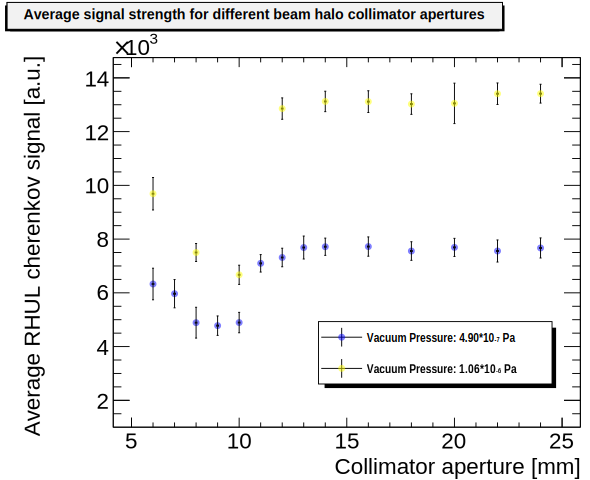
\includegraphics[width=\textwidth]{AverageSignal_perAperture_VacuumPressures.pdf}
\caption[RHUL Cherenkov detector signal vs. collimator aperture: different vacuum pressures]{Average signal as a function of the full aperture of the vertical beam halo collimator. The signal was measured for a beam intensity of \num{0.5e10} and a PMT voltage of \SI{900}{\volt}. The vacuum pressure was lowered from \SI{4.9e-7}{\pascal} to \SI{1.06e-6}{\pascal}. For each aperture, 500 ADC pulses were recorded, and the signal was averaged over the number of pulses. The error bars to the mean values are the standard deviation of the signal distributions at each point.}
\label{fig:AverageSignal_Aperture_VacuumPressures}
\end{figure}
\subsubsection{Test collimator alignment wrt beam position}
\begin{figure}
\centering
\includegraphics[width=\textwidth]{AverageSignal_perJawPosition.pdf}
\caption[RHUL Cherenkov detector signal vs. collimator half aperture]{Average signal as a function of the position of the upper/lower jaw of the vertical beam halo collimator. The signal was measured for a beam intensity of \num{1.05e10} and a PMT voltage of \SI{800}{\volt}. First, the lower jaw was fixed to its open position (\SI{12}{\milli\metre}) and the upper jaw was moved to the positions plotted, then vice versa. For each jaw position, 500 ADC pulses were recorded, and the signal was averaged over the number of pulses. The error bars to the mean values are the standard deviation of the signal distributions at each point.}
\label{fig:AverageSignal_HalfAperture}
\end{figure}
\begin{figure}
\begin{subfigure}[b]{0.5\textwidth}
\includegraphics[width=\textwidth]{AsymmetricScan_4mm_beamintensity084_lego.pdf}
\end{subfigure}
\begin{subfigure}[b]{0.5\textwidth}
\includegraphics[width=\textwidth]{AsymmetricScan_4mm_beamintensity084_colz.pdf}
\end{subfigure}
\caption[RHUL Cherenkov detector signal for certain upper/lower jaw positions]{Average signal as a function of the position of the upper and lower jaw of the vertical beam halo collimator. The signal was measured for a beam intensity of \num{0.84e10} and a PMT voltage of \SI{900}{\volt}. The jaws were moved simultaniously around \SI{4}{\milli\metre}. For each jaw position, at least 500 ADC pulses were recorded, and the signal was averaged over the number of pulses. The content of the bins were set to the appropriat average signal strength at that point.}
\label{fig:AverageSignal_Asymmetric}
\end{figure}
%---------------------------------------------------
\subsection{Collimator as background source}
\label{sec:BDSIM_sim}
\subsection{Effect on background level at IP}

%---------------------------------------------------
\section{Background from a Muon Spoilers}
\subsection{MUCARLO}
